%\documentclass[a4paper]{article}
%% Language and font encodings
\documentclass[twocolumn,aps,prl]{revtex4-1}
\usepackage[utf8]{inputenc}
\usepackage[spanish, es-tabla]{babel}
\usepackage[T1]{fontenc}
\usepackage{amsmath}
\usepackage{amssymb}
\usepackage{siunitx}
\usepackage{multirow}
\usepackage{float}
\usepackage{enumitem} % enumerar

\sisetup{math-micro=\text{µ},text-micro=µ}

\usepackage[toc,page]{appendix}

%% Sets page size and margins
\usepackage[a4paper,top=1.5cm,bottom=2cm,left=1.7cm,right=1.7cm,marginparwidth=1.75cm]{geometry}

%% Sets caption text size(its bigger than text)
\usepackage{caption}
\captionsetup[figure]{font=small}
\usepackage{subcaption}

%% Useful packages
\usepackage{svg}
\usepackage{epstopdf}
\usepackage{amsmath}
\usepackage{graphicx}
\usepackage[colorlinks=true, allcolors=blue]{hyperref}

\newcommand{\nstar}{n^*} 
\newcommand{\Nstar}{N^*} 

\newcommand*\sepline{%
  \begin{center}
    \rule[1ex]{.5\textwidth}{.5pt}
  \end{center}}

%%%%%%%%%%%%%%%%%%%%%%%%%%%%%%%%%%%%%%%%%%%%%%%%%%%%%%
%%%%%%%%%%%%%%%%%%%%%%%%%%%%%%%%%%%%%%%%%%%%%%%%%%%%%%

\begin{document}

% ██   ██ ███████  █████  ██████
% ██   ██ ██      ██   ██ ██   ██
% ███████ █████   ███████ ██   ██
% ██   ██ ██      ██   ██ ██   ██
% ██   ██ ███████ ██   ██ ██████

\title{Práctico 5}
\author{M. G. Aramayo}
\affiliation{Matemática de sistemas biológicos, Instituto Balseiro}

% \begin{abstract}
% Mete acá las conclusiones.
% \end{abstract}

\maketitle


\section{Resolución Ej 1}
% ███████╗██╗  ██╗ ██╗
% ██╔════╝╚██╗██╔╝███║
% █████╗   ╚███╔╝ ╚██║
% ██╔══╝   ██╔██╗  ██║
% ███████╗██╔╝ ██╗ ██║
% ╚══════╝╚═╝  ╚═╝ ╚═╝

%**********
\begin{figure*}[ht!]
  \begin{subfigure}[b]{0.49\linewidth}
    \centering
      \centering
      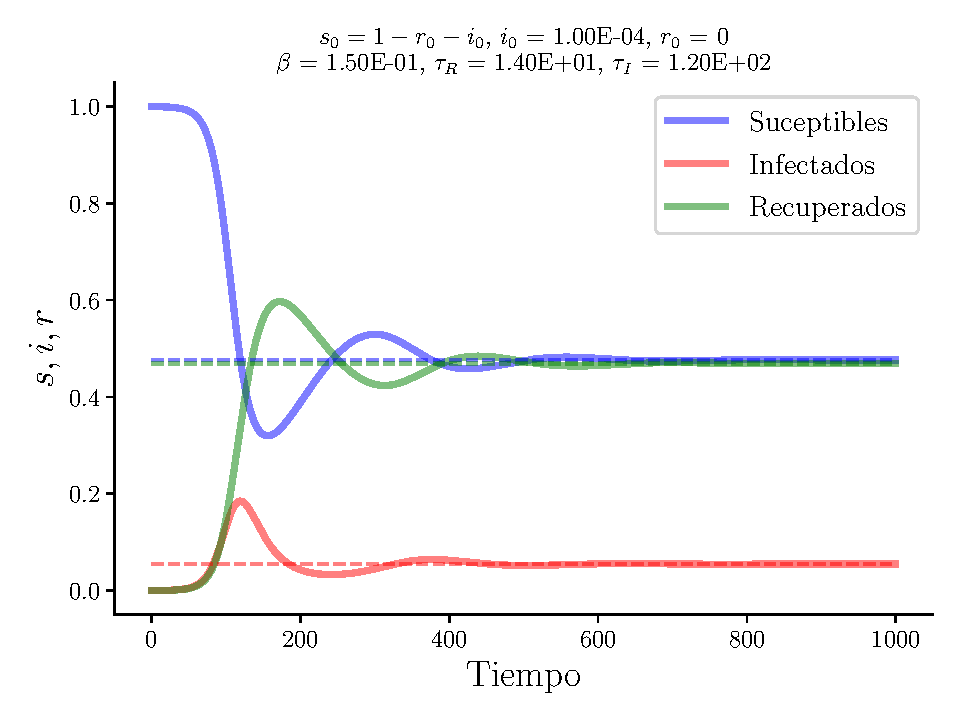
\includegraphics[width = 1.05\textwidth]{figuras/ex01-a-sir.pdf}
      \caption{}
      \label{fig:ex01-a-sir}
  \end{subfigure}\quad
  \begin{subfigure}[b]{0.49\linewidth}
      \centering
      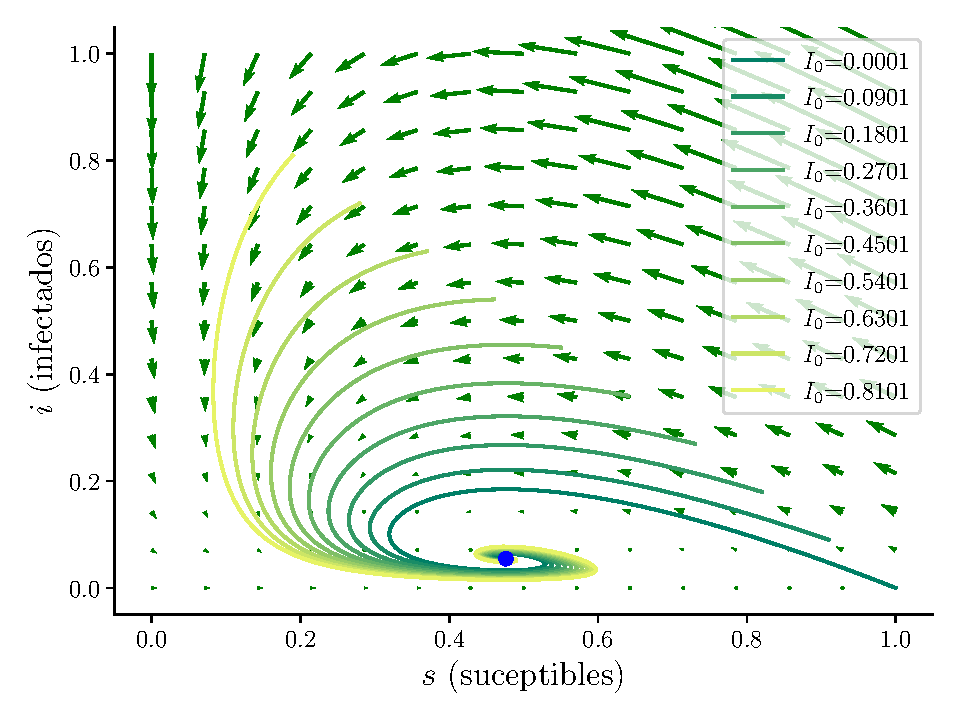
\includegraphics[width = 1.05\textwidth]{figuras/ex01-a-vector.pdf}
      \caption{}
      \label{fig:ex01-a-vector}
  \end{subfigure}\quad
  % \end{figure*}

  % \begin{figure*}[ht!]
  \begin{subfigure}[b]{0.49\linewidth}
      \centering
      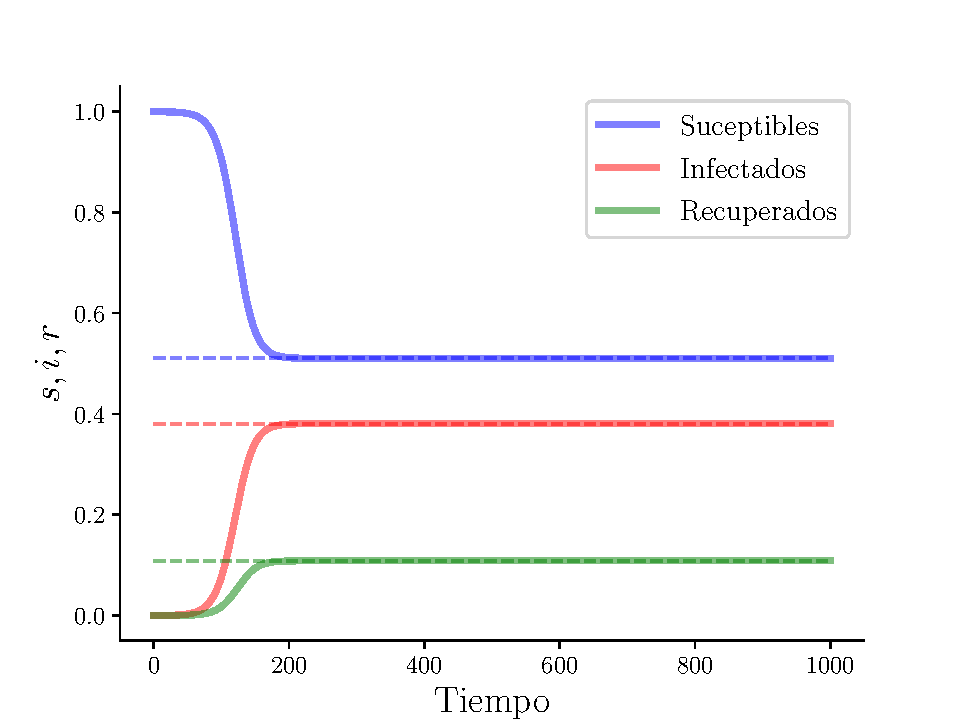
\includegraphics[width = 1.05\textwidth]{figuras/ex01-b-sir.pdf}
      \caption{}
      \label{fig:ex01-b-sir}
  \end{subfigure}\quad
  \begin{subfigure}[b]{0.49\linewidth}
      \centering
      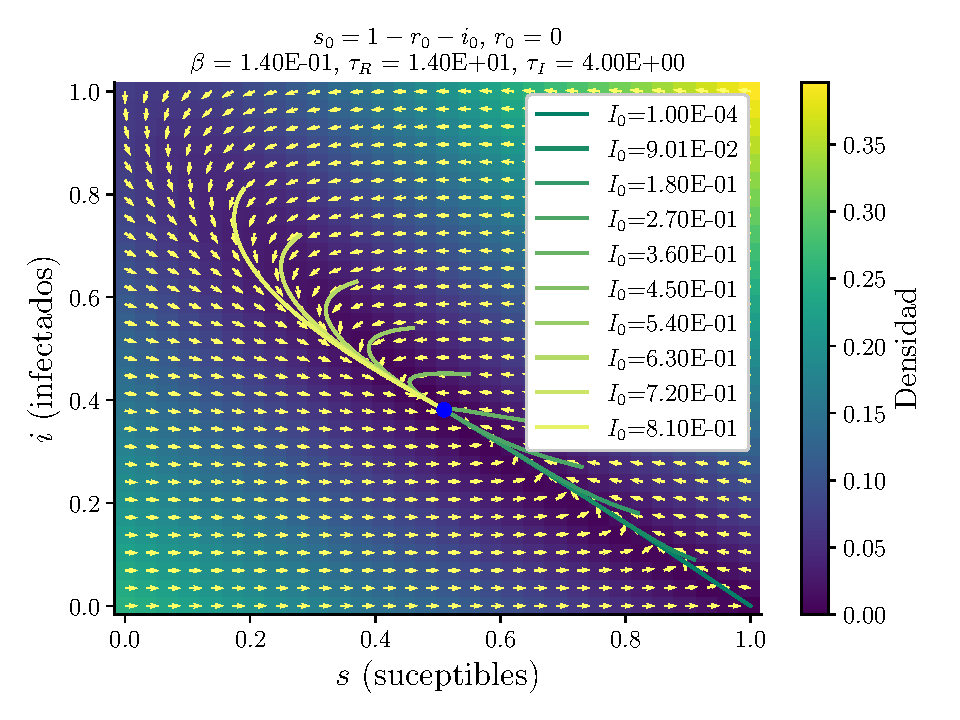
\includegraphics[width = 1.05\textwidth]{figuras/ex01-b-vector.pdf}
      \caption{}
      \label{fig:ex01-b-vector}
  \end{subfigure}\quad
  % \end{figure*}

  % \begin{figure*}[ht!]
  \begin{subfigure}[b]{0.49\linewidth}
      \centering
      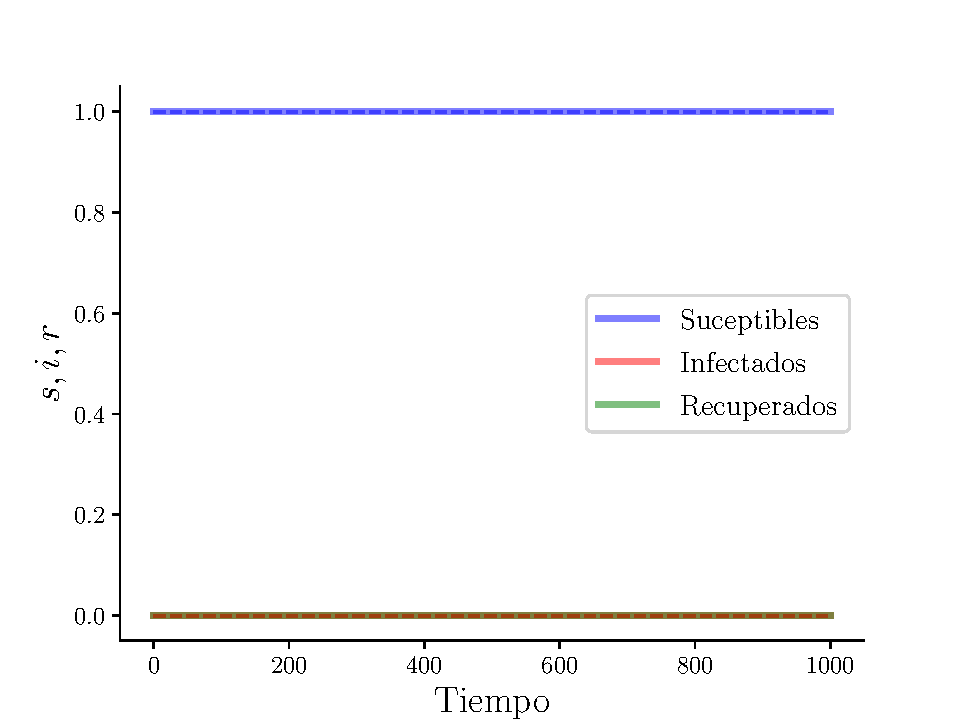
\includegraphics[width = 1.05\textwidth]{figuras/ex01-c-sir.pdf}
      \caption{}
      \label{fig:ex01-c-sir}
  \end{subfigure}\quad
  \begin{subfigure}[b]{0.49\linewidth}
      \centering
      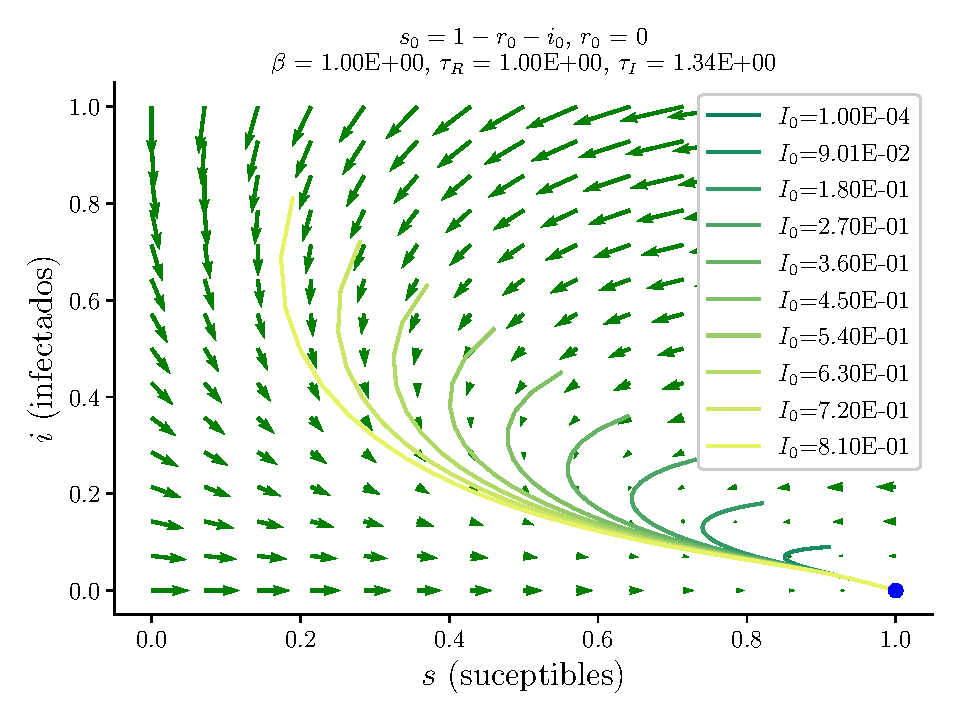
\includegraphics[width = 1.05\textwidth]{figuras/ex01-c-vector.pdf}
      \caption{}
      \label{fig:ex01-c-vector}
  \end{subfigure}\quad
  \caption{Solución de las ecuaciones sir para distintas condiciones iniciales y parametros.}
  \label{fig:ex01}
\end{figure*}

Se analiza el modelo epidemiológico SIR, dado por el sistema dinámico:
$$
\left\lbrace
\begin{aligned}
\frac{d s}{d t} & = f_1(s,i,r) = -\beta s i+\frac{1}{\tau_{R}} r \\
\frac{d i}{d t} & = f_2(s,i,r) =\beta s i-\frac{1}{\tau_{I}} i \\
\frac{d r}{d t} & = f_3(s,i,r) =\frac{1}{\tau_{I}} i-\frac{1}{\tau_{R}} r
\end{aligned}
\right.
$$
a población constante, por lo que: $s+i+r =1 $, se tiene una solución a este sistema en la Fig. \ref{fig:ex01}.

Los equilibrios del sistema $\left(s^{*}, i^{*}, r^{*}\right)$ se obtienen mediante:
$$
\left\lbrace
\begin{aligned}
f_1(s^*, i^*, r^*) &= 0  \\
f_2(s^*, i^*, r^*) &= 0  \\
f_3(s^*, i^*, r^*) &= 0
\end{aligned}
\right.
\Rightarrow
\left\lbrace
\begin{aligned}
\beta s^* i^* = \frac{1}{\tau_{R}} r^* \\
\beta s^* i^* = \frac{1}{\tau_{I}} i^* \\
\frac{1}{\tau_{I}} i^* = \frac{1}{\tau_{R}} r^*
\end{aligned}
\right.
\Rightarrow
\left\lbrace
\begin{aligned}
i^* &= \frac{\tau_{I}}{\tau_{R}} r^* \\
s^* &= \frac{1}{\tau_{I} \beta}      \\
i^* &= \frac{\tau_{I}}{\tau_{R}} r^* 
\end{aligned}
\right.
$$
, con $i \neq 0$

El sistema anterior y la población constante implica que:
$$
i^{*} \quad=\frac{\beta \tau_{I}-1}{\beta\left(\tau_{l}+\tau_{R}\right)}
$$

% No se pierde mucho descartando $i^{*}=0$, ese equilibrio no tiene dinámica.

El equilibrio queda:
$$
\left\lvert 
\begin{aligned}
      % P_1 &= (1, 0, 0) \\ 
    P_2 &= 
    ( \frac{1}{\tau_{I} \beta}  
    , \frac{\beta \tau_{I}-1}{\beta\left(\tau_{l}+\tau_{R}\right)}
    , \frac{\tau_{R}}{\tau_{I}} \frac{\beta \tau_{I}-1}{\beta\left(\tau_{l}+\tau_{R}\right)}
    ) \\ 
\end{aligned} \right.
$$


Mediante un análisis lineal es posible demostrar que el sistema presenta oscilaciones amortiguadas. 

Con la condición de población constante es posible reducir el sistema a uno bidimesional:
$$ \left\lbrace
\begin{aligned}
\frac{d s}{d t} &= f_1(s, i) = \beta s i - \frac{1}{\tau_{R}} (s+i) +  \frac{1}{\tau_{R}}   , \\
\frac{d i}{d t} &= f_2(s, i) = \beta s i-\frac{1}{\tau_{I}} i  
\end{aligned}
\right.
$$
Con su correspondiente matriz Jacobiana:
$$
J (s, i) = 
\left(
  \begin{array}{cc}
-\beta i - \frac{1}{\tau_{R}} & -\beta s - \frac{1}{\tau_{R}} \\
 \beta i                     &   \beta s - \frac{1}{\tau_{I}}
  \end{array}
\right)
$$
el análisis lineal requiere obtener los autovalores $\lambda_{1,2}$ de la matriz Jacobiana del sistema, la ecuación característica resulta:
% \sepline
% $$
% J_2 = 
% \left(
%   \begin{array}{cc}
%     \frac{-\beta\tau_{I}\tau_{R}-\tau_{I}}{\tau_{R}\left( \tau_{I}+\tau_{R} \right)} & -\frac{1}{\tau_I}-\frac{1}{\tau_R} \\
%     \frac{\beta \tau_I-1}{\tau_I + \tau_R}              &   0
%   \end{array}
% \right)
% $$
% $bd = -\frac{\beta \tau_I -1}{ \tau_I \tau_R}$
% \sepline
$$
\begin{aligned}
  0 & = \lambda^{2} \\
  \quad & +\lambda\left(\beta i^{*}+\frac{1}{\tau_{R}}-\beta s^{*}+\frac{1}{\tau_{I}}\right) \\
  \quad & +\left(\frac{\beta i^{*}}{\tau_{I}}-\frac{\beta s^{*}}{\tau_{R}}+\frac{1}{\tau_{I} \tau_{R}}+\frac{\beta i^{*}}{\tau_{R}}\right)
\end{aligned}
$$

Para el punto $P_2$, la ecuación característica es
$$
\lambda^{2}+\lambda\left(\frac{\beta \tau_{I}-1}{\tau_{l}+\tau_{R}}+\frac{1}{\tau_{R}}\right)+\left(\frac{\beta \tau_{l}-1}{\tau_{l} \tau_{R}}\right) \quad=0, 
$$
y las soluciones, $\lambda_{1, 2}$ son:
$$
\begin{aligned}
  \lambda_{1,2} =
  & \frac{1}{2} \left[-
  \left(\frac{\beta \tau_{l}-1}{\tau_{I}+\tau_{R}}+\frac{1}{\tau_{R}}\right)  \right.\\
  &
  \left.
  \pm \sqrt{\left(\frac{\beta \tau_{I}-1}{\tau_{I}+\tau_{R}}+\frac{1}{\tau_{R}}\right)^{2}-4\left(\frac{\beta \tau_{I}-1}{\tau_{I} \tau_{R}}\right)} \right]
\end{aligned}
$$
% y corresponden a los dos autovalores que buscamos. El término fuera de la raíz es negativo, dado que:
% $$
% \left(\frac{\beta \tau_{I}-1}{\tau_{I}+\tau_{R}}+\frac{1}{\tau_{R}}\right) \quad>0
% $$
% Tras un poco de álgebra, se desprende que esta condición se cumple si y sólo si:
% $\beta \tau_{R} \quad>-1$
% esto siempre es cierto porque $\beta$ y $\tau_{R}$ son números reales del mismo signo.

% No podemos afirmar a que para cualquier valores de los parámetros estos autovalores son imaginarios o reales. Si son imaginarios, tendremos dos autovalores complejos conjugados de parte real negativo, lo cual corresponde a una espiral estable en el espacio de fases. En cambio, si el discriminante es cero, tendremos un único autovalor negativo, lo cual implica la existencia de un nodo degenerado estable. Finalmente, si el discriminante es mayor a cero, tendremos dos autovalores reales de distinto signo, con lo cual habrá un saddle.

% A continuación, mostramos un valor de parámetros que cumple cada una de estas condiciones y el valor correspondiente del determinante con su signo. Primero, graficaremos el diagrama de fases en torno al punto de equilibrio, como una manera de constatar computacionalmente que el resultado del análisis lineal es correcto. Allí, dibujaremos también algunas trayectorias del sistema para diferentes condiciones iniciales arbitrarias. Adicionalmente, señalamos el punto de equilibrio correspondiente con un punto azul.

y corresponden a los dos autovalores que buscamos. El término fuera de la raíz es negativo, dado que:
$$
\left(\frac{\beta \tau_{l}-1}{\tau_{I}+\tau_{R}}+\frac{1}{\tau_{R}}\right) 
% \quad> 
\stackrel{>}{<} 0
$$
Reordenando se obtiene:
$$
\beta \tau_{R}
% \quad> 
\stackrel{>}{<} -1
$$
Como ambos son valores positivos 
$$
\beta \tau_{R}
> -1
$$
Si propagamos la desigualdad
$$
\left(\frac{\beta \tau_{l}-1}{\tau_{I}+\tau_{R}}+\frac{1}{\tau_{R}}\right) 
> 0
$$
lo cual implica que que los autovalores complejos tienen siempre parte real negativa, la raíz, en caso de tener radicando negativo es un numero complejo. Esto implica que cuando se tienen oscilaciones siempre se amortiguan. 

\section{Resolución Ej 2}
% ███████╗██╗  ██╗    ██████╗  
% ██╔════╝╚██╗██╔╝    ╚════██╗
% █████╗   ╚███╔╝      █████╔╝
% ██╔══╝   ██╔██╗     ██╔═══╝ 
% ███████╗██╔╝ ██╗    ███████╗
% ╚══════╝╚═╝  ╚═╝    ╚══════╝

\begin{figure*}[!ht]
  \centering
    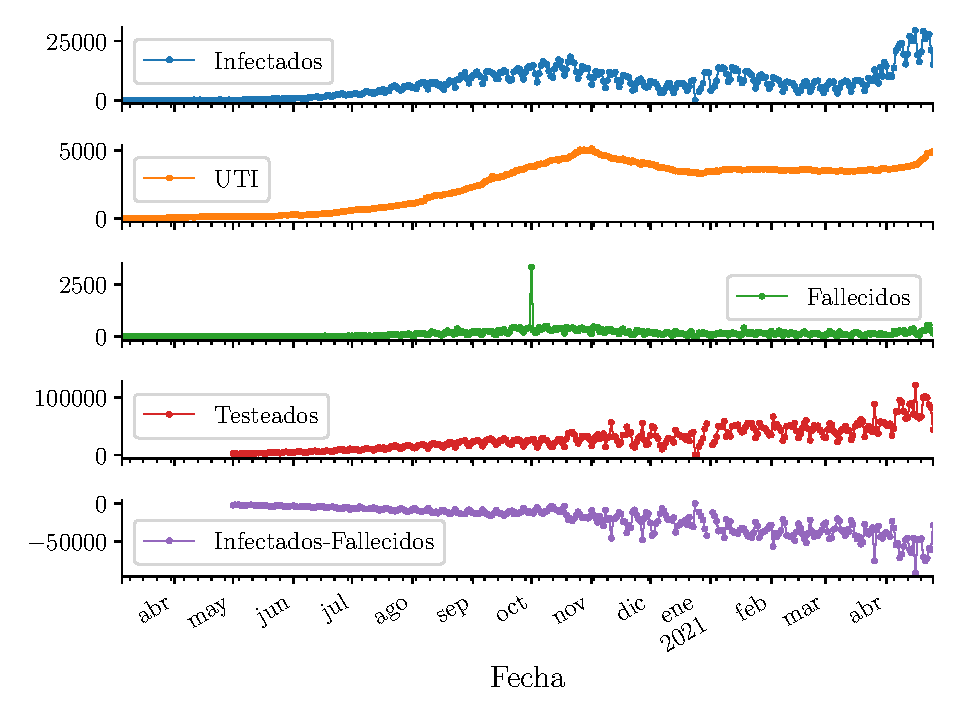
\includegraphics[width = 0.8\textwidth]{figuras/ex02-resumen.pdf}
    \caption{Cosa}
    \label{fig:ex02Resumen}
\end{figure*}

En la Fig. \ref{fig:ex02Resumen} se tiene un gráfico que resume, numero de infectados, de fallecidos, de testeados y de UTI(Unidad de terapia intensiva).

\begin{figure*}[ht!]
  \centering
  \begin{subfigure}[b]{0.49\linewidth}
      \centering
      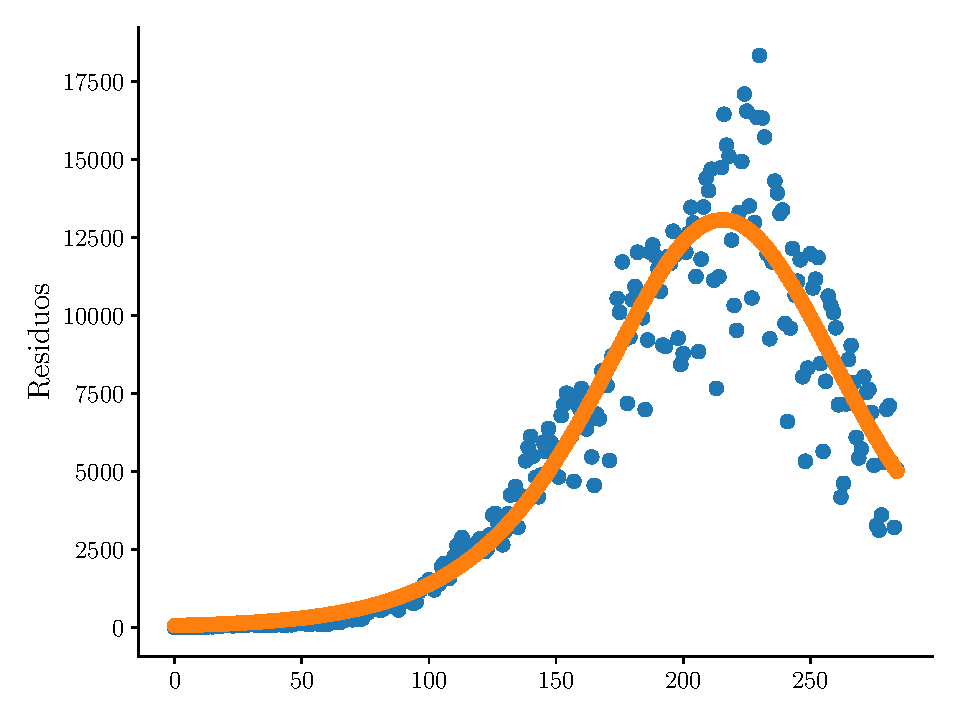
\includegraphics[width = 1.05\textwidth]{figuras/ex02-fit.pdf}
      \caption{}
      \label{fig:ex02-fit}
  \end{subfigure}\quad
  \begin{subfigure}[b]{0.49\linewidth}
      \centering
      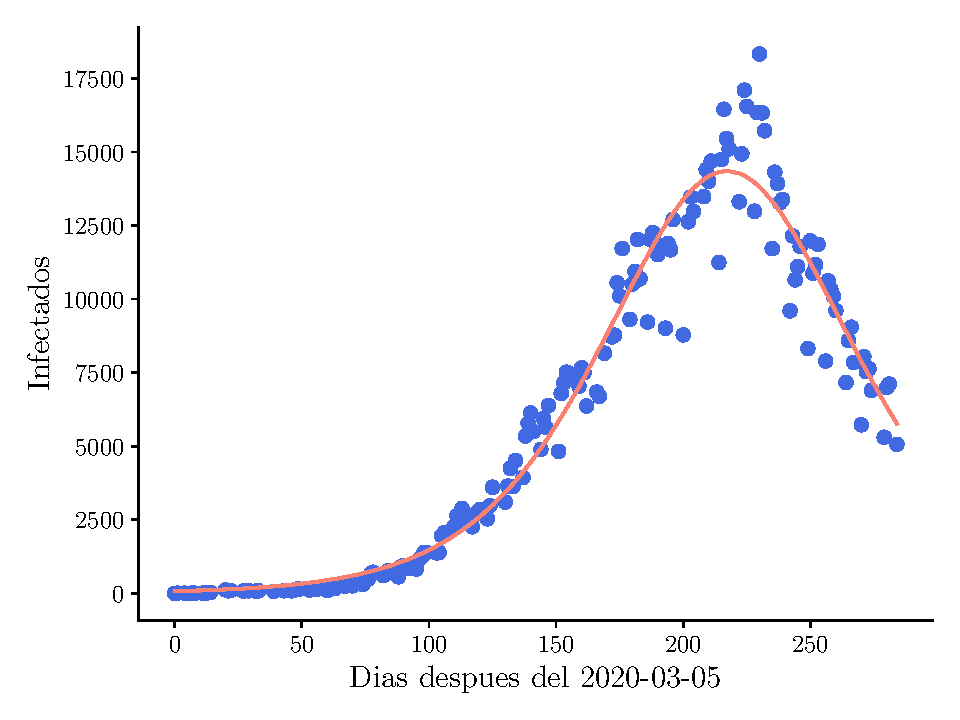
\includegraphics[width = 1.05\textwidth]{figuras/ex02-fit-sin-Finde.pdf}
      \caption{}
      \label{fig:ex02-fit-sin-Finde}
  \end{subfigure}
  \caption{De izquierda a derecha, datos originales y datos sin feriados ni fines de semana respectivamente con sus respectivos ajustes de la Ec. \ref{eq:pico}.}
  \label{fig:ex02-fit-ambas}
\end{figure*}

Se observa con cierta frecuencia una caida en infectados. Esto se debe a que los fines de semanas se realizan menos tests. Para el resto del analisis se omiten estos dias junto con los dias feriados de los año 2020 y 2021. En las Fig. \ref{fig:ex02-fit-ambas} a \ref{fig:ex02-residuos-ambas}

Es posible realizar un ajuste a los picos de infectados mediante:

\begin{equation} \label{eq:pico}
  a \operatorname{sech} ^2 \left( bt + c \right).
\end{equation}

El pico que figura en los datos sin feriados y fines de semana, ocurre el \textbf{2020-10-21}. Tomando datos desde el \textbf{2020-03-05}, se predice que la fecha del pico es \textbf{2020-10-08} luego de 168 dias(24 semanas) de datos. Por esto, se predice la fecha del primer pico con 62 dias de antelacion y con un error de 13 dias. En la Fig. \ref{fig:ex02Resumen}, se tienen las predicciones que se obtienen para disintos numeros de semanas de datos sobre los cuales se realiza el ajuste. 



\begin{figure*}[ht!]
  \begin{subfigure}[b]{0.49\linewidth}
      \centering
      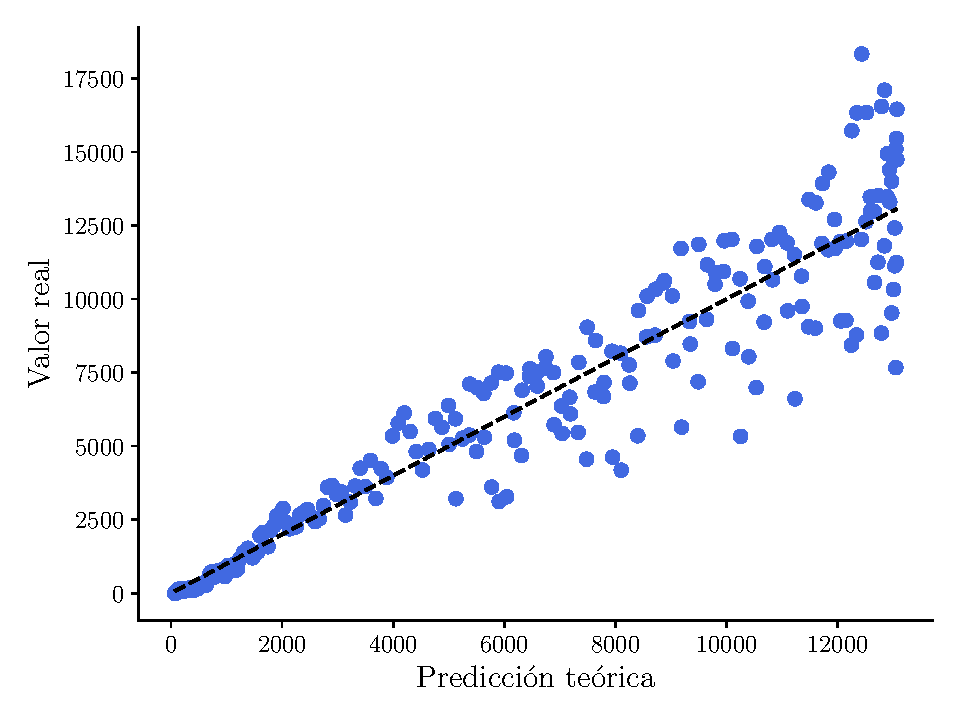
\includegraphics[width = 1.05\textwidth]{figuras/ex02-qq.pdf}
      \caption{}
      \label{fig:ex02-qq}
  \end{subfigure}\quad
  \begin{subfigure}[b]{0.49\linewidth}
      \centering
      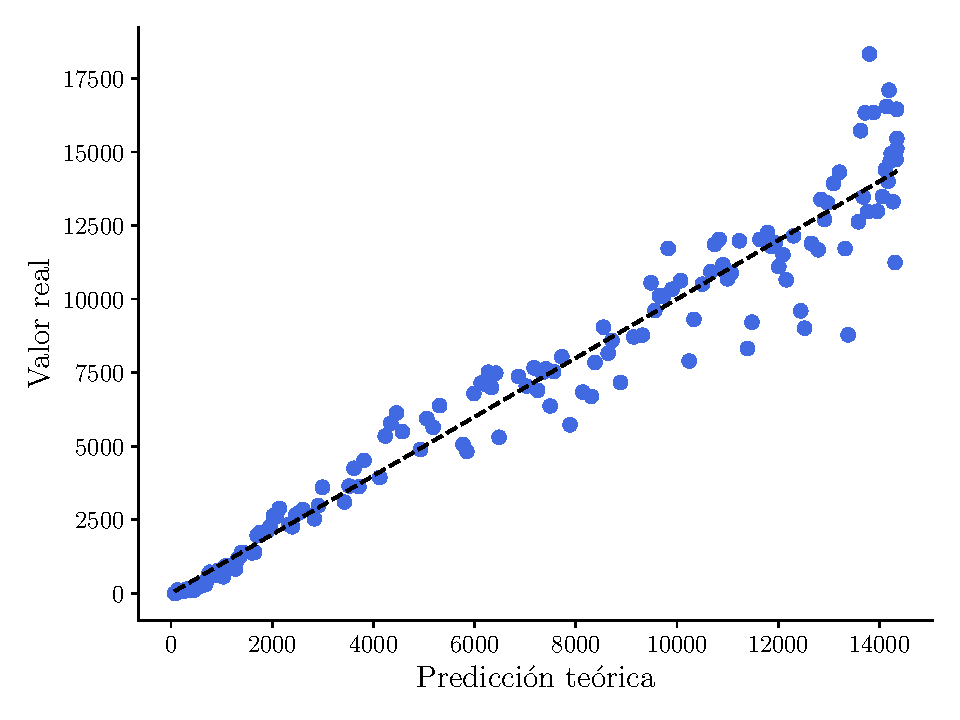
\includegraphics[width = 1.05\textwidth]{figuras/ex02-qq-sin-Finde.pdf}
      \caption{}
      \label{fig:ex02-qq-sin-Finde}
  \end{subfigure}
  \caption{De izquierda a derecha, curvas Q-Q a partir de los datos originales y a partir de los datos excluyendo feriados y fines de semanas.}
  \label{fig:ex02-qq-ambas}
\end{figure*}

\begin{figure*}[ht!]
  \begin{subfigure}[b]{0.49\linewidth}
      \centering
      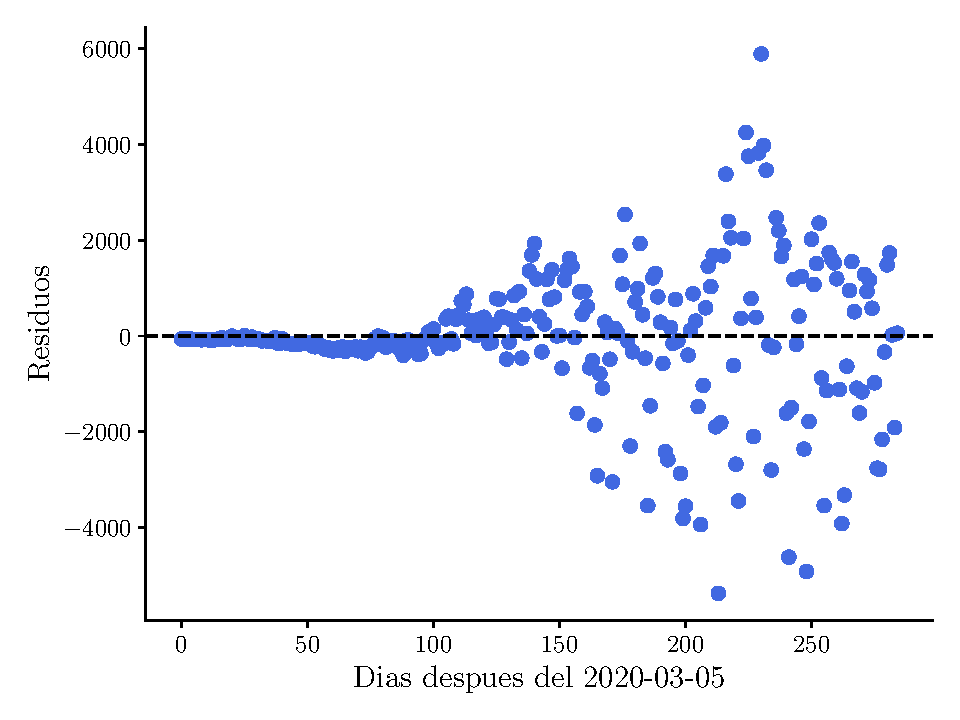
\includegraphics[width = 1.05\textwidth]{figuras/ex02-residuos.pdf}
      \caption{}
      \label{fig:ex02-residuos}
  \end{subfigure}\quad 
  \begin{subfigure}[b]{0.49\linewidth}
      \centering
      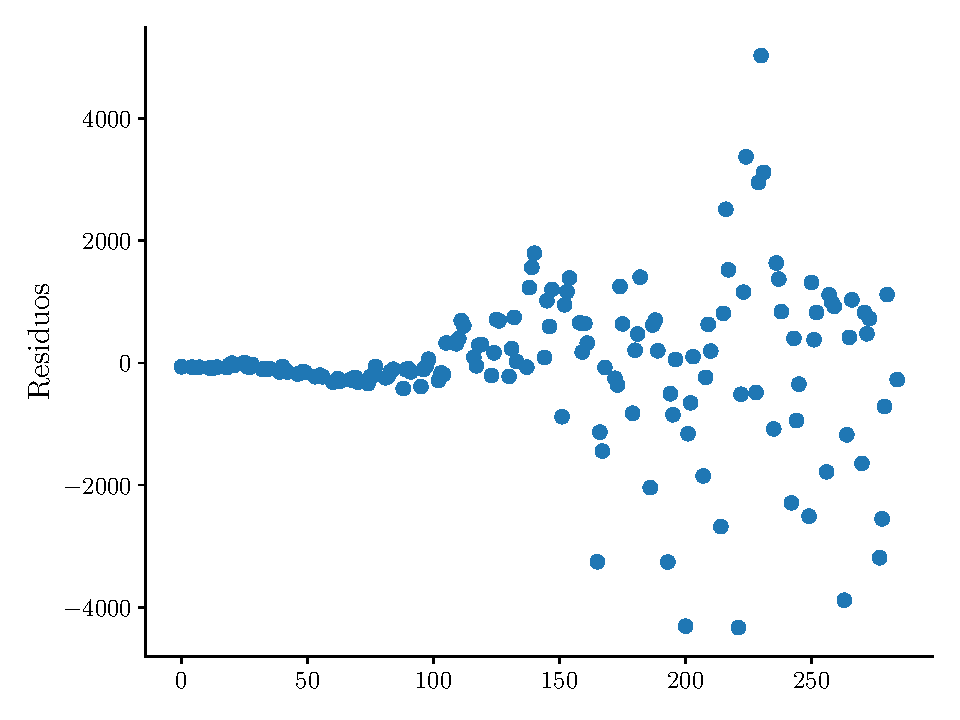
\includegraphics[width = 1.05\textwidth]{figuras/ex02-residuos-sin-Finde.pdf}
      \caption{}
      \label{fig:ex02-residuos-sin-Finde}
  \end{subfigure}
  \caption{De izquierda a derecha, residuos del ajuste de la Ec. \ref{eq:pico} a partir de los datos originales y a partir de los datos excluyendo feriados y fines de semanas.}
  \label{fig:ex02-residuos-ambas}
  %\label{fig:ex02-residuos-sin-Finde}
\end{figure*}

\begin{figure*}[ht!]
  \centering
      \centering
      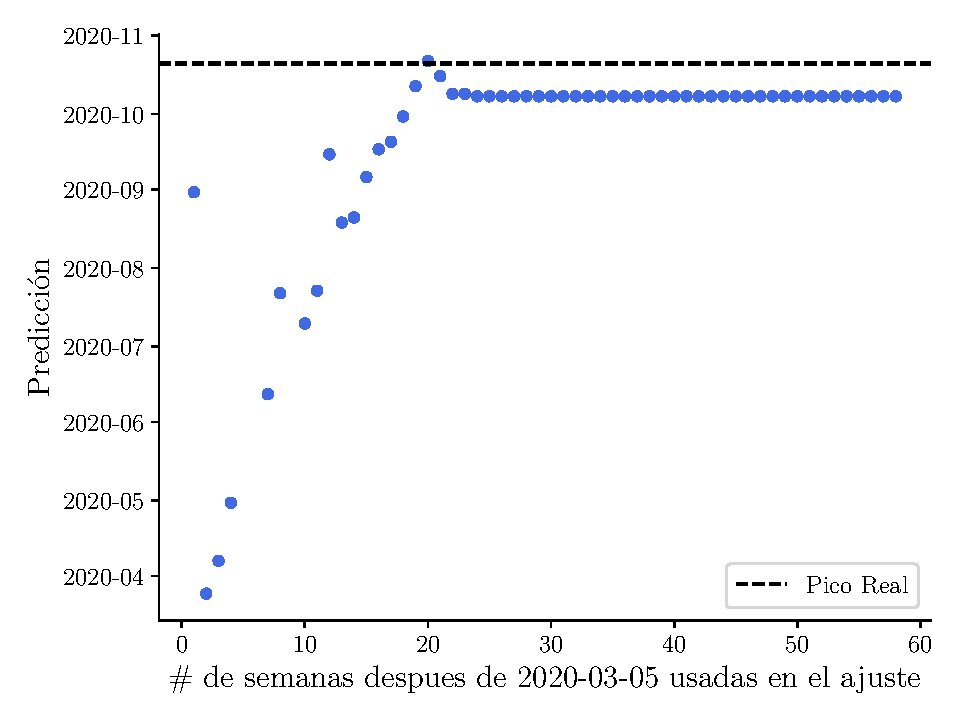
\includegraphics[width = 0.55\textwidth]{figuras/ex02-prediccion-semanas.pdf} 
      % \caption{}
      \caption{Predicción de la fecha del pico vs. cuantas semanas de datos se usan en el ajuste de la Ec. \ref{eq:pico}.}
      \label{fig:ex02-semanas}
\end{figure*}

\end{document}
